\section{Project Plan}
\label{sec:projectplan}
To provide a schedule and to check whether the project is still proceeding on a good pace, a project plan has been developed after performing the requirements analysis and discussing various aspects of the project with the client (the main author of the paper summarised in \autoref{sub:statistical_model_selection}). This project plan can be found as a Gantt-Chart in \autoref{fig:projectplan}. Further details of it can be seen in \autoref{fig:projectplan:details:1} and \autoref{fig:projectplan:details:2}. In general, light blue colour is used for tasks related to the actual thesis (writing, reports, research). Blue coloured tasks represent requirement, analysis and development tasks. Light green tasks are related to project reports whereas dark-green tasks stand for feedback cycles. Green milestones (diamonds) represent internal release candidates of the development iterations. Red milestones represent external milestones and due dates. 

This schedule will be updated over time according to the actual progress of the project.

\begin{sidewaysfigure}[h]
	\centering
	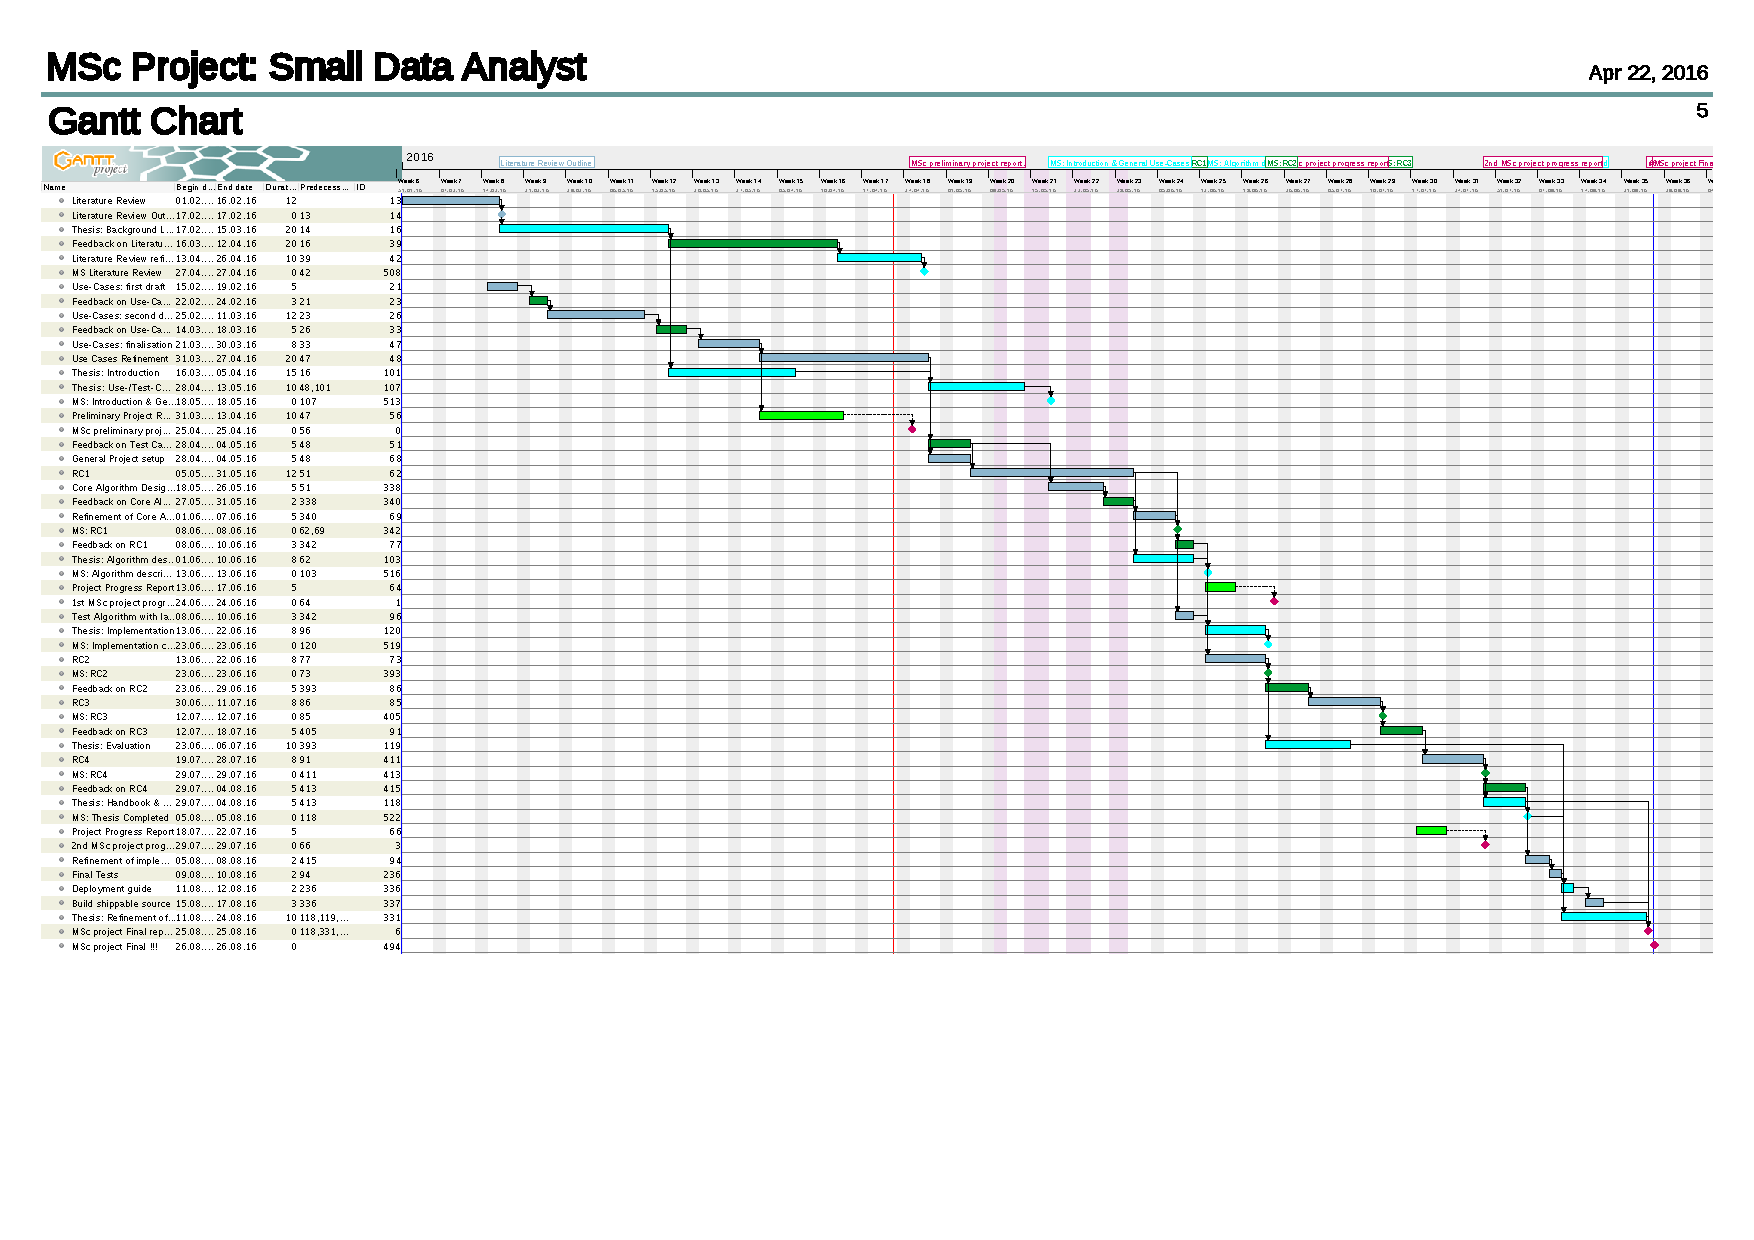
\includegraphics[page=1,width=\textwidth]{appendix/Projectplan.pdf}
	\caption{Project plan for the whole development and research}
	\label{fig:projectplan}
\end{sidewaysfigure}

\begin{sidewaysfigure}[h]
	\centering
	\includegraphics[page=2,width=\textwidth]{appendix/Projectplan.pdf}
	\caption{Detailed description and properties of single task listed in the project plan (Page 1/2)}
	\label{fig:projectplan:details:1}
\end{sidewaysfigure}

\begin{sidewaysfigure}[h]
	\centering
	\includegraphics[page=3,width=\textwidth]{appendix/Projectplan.pdf}
	\caption{Detailed description and properties of single task listed in the project plan (Page 2/2)}
	\label{fig:projectplan:details:2}
\end{sidewaysfigure}
